\documentclass{article}
\usepackage[utf8]{inputenc}
\usepackage{graphicx}
\usepackage{epstopdf}
\usepackage{caption}
\usepackage{subcaption}
\usepackage{multirow}
\usepackage{hyperref}
\usepackage{url}
\usepackage{seqsplit}
\hypersetup{pdfstartview={FitH null null null}}
\usepackage{amssymb,amsmath}
\usepackage{amsthm}
\usepackage{empheq}
\usepackage{algorithm,algpseudocode}
\usepackage[margin=1.5in]{geometry}
\usepackage{listings}
\usepackage{program}
\lstset{language=Python} 

\usepackage{listings}
\usepackage{color} %red, green, blue, yellow, cyan, magenta, black, white
\definecolor{mygreen}{RGB}{28,172,0} % color values Red, Green, Blue
\definecolor{mylilas}{RGB}{170,55,241}


\title{Comparison of protein-protein docking prediction and optimization methods}
\author{Caiwei Wang, Xiaokai Qian, Sean Lander, \\Haipei Fan, Puneet Gaddam, Brett Koonce\\\\University of Missouri - Columbia}

\date{April 7, 2014}

\algloopdefx{NoEndIf}[1]{\textbf{If} #1 \textbf{then}}

\begin{document}

\maketitle

\section{Abstract}



\section{Introduction}



\section{Methods}



\subsection{Pipeline}

\begin{figure}[H]
\begin{center}
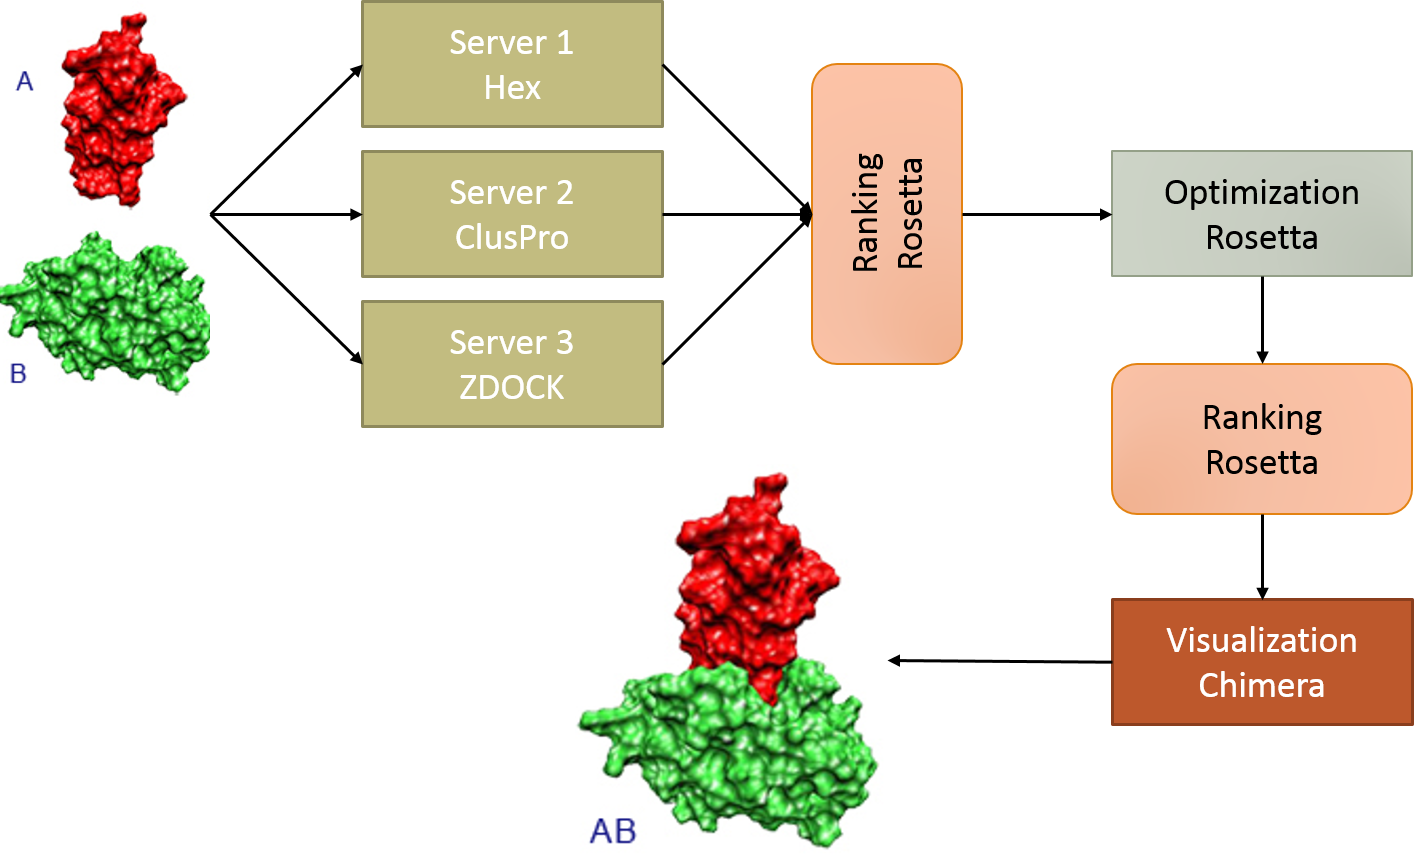
\includegraphics[width=\textwidth]{pipeline}
\caption{An overview of the comparison pipeline}
\label{Fig:blosum}
\end{center}
\end{figure}

\begin{enumerate}
\item Decoy Creation:
Decoys are created using an ensemble of docking servers. This list can be extended beyond the servers listed, as well as include locally created predictions.

\item Ranking:
RosettaDock's prediction scoring is used to normalize the results, as each tool uses its own scoring and ranking system. The decoys are then ranked based on their new scores and the top 10 continue on for optimization.

\item Optimization:
Once again RosettaDock is used, this time for its optimization capabilities. The top 10 decoys are fed into Rosetta and the results are fed into a second round of scoring.

\item Final Selection and Scoring:
The optimized decoys are scored by RosettaDock once again and ranked accordingly. The top scoring model is chosen as the best candidate.

\item Visualization:
Chimera is used to visualize the best model overlaid with the native conformation, as well as the top 10 before and after optimization.
\end{enumerate}

\subsection{CAPRI Target and Docking Tool Selection}

We selected the following template-free targets from the CAPRI database to build a model for: T53, T50. These targets were chosen due to their high predictability by many of the tools used, allowing for a balanced comparison of predictive capacity on easy targets.

The tools selected represent some of the different methods currently employed for docking prediction and rankings - Fast Fourier Transforms, Spherical Polar Fourier, filter by clustering and data-driven rankings - as well as how base decoys compare to their optimized counterparts. 

\subsection{Pre-Processing}

\subsection{Decoy Creation}

\subsubsection{Hex}

\subsubsection{ClusPro}

\subsubsection{ZDOCK}
ZDOCK uses a mixture of Fast Fourier Transform and data-driven scoring/ranking in order to create and sorts its decoy. While this allows for very fast decoy creation, it results in a stochastic algorithm, so multiple runs will always generate the same results. The ZDOCK server produces 500 decoys on a run, but only the top 10 of those are available for download, making it hard to build up an appropriately sized sample group.

\subsection{Decoy Optimization}

\begin{enumerate}

\item Decoy Ranking

\item Optimization

\end{enumerate}



\section{Results}

\subsection{Interface Creation}

\subsection{Scoring Methods - RMSD vs RosettaDock}

\begin{enumerate}

\item Before Optimization

\item After Optimization

\end{enumerate}

\subsection{Visualization}



\section{Conclusion}



\section{Citations}

We thank the following tools and papers: \\\\



\end{document}


\end{document}
